% ======================================================================
% Journal of Computer-Aided Molecular Design (2026)
% Short Communication - V6.1 (Revised per Reviewer 2, Round 2)
% ======================================================================
\documentclass[global,twocolumn]{svjour}

\usepackage[T1]{fontenc}
\usepackage{amsmath}
\usepackage{graphicx}
\usepackage{booktabs}
\usepackage{array}
\usepackage{microtype}
\usepackage{xurl}
\usepackage[numbers,sort&compress]{natbib}
\usepackage[colorlinks=true,linkcolor=blue,citecolor=blue,urlcolor=blue]{hyperref}
\usepackage{caption}

\journalname{Journal of Computer-Aided Molecular Design}
\newcommand{\st}{\footnotesize\setlength{\tabcolsep}{3pt}}

\begin{document}

\title{Cognate redocking as a quality-control step for cryo-EM kinase
       receptor structures: a study of ATR/CHK1 and
       CDK-activating kinase}
\titlerunning{Cognate redocking for cryo-EM kinase structures}

\author{Authors to be added}
\authorrunning{Authors to be added}
\institute{Affiliation to be added}
\offprints{}

\date{Received: / Accepted:}
\maketitle

% ======================================================================
\begin{abstract}
Cognate redocking---reproducing a receptor's own deposited experimental
ligand model---is a standard quality-control step in structure-based virtual
screening. Two recent cryo-EM structures of ATR (PDB~9L40, 2.87~\AA{}, bound
to berzosertib; PDB~9L4B, 3.20~\AA{}, bound to camonsertib) were tested under
an identical AutoDock Vina protocol (exhaustiveness~32, three seeded
replicates, 2.0~\AA{} symmetry-corrected RMSD pass threshold). 9L4B passed
(0.61$\pm$0.02~\AA{}) whereas the higher-resolution 9L40 failed
(2.53$\pm$0.01~\AA{}). A sensitivity analysis using 18, 22, 26, and
30~\AA{} search boxes confirmed the failure is not an artifact of box size.
Extending the identical protocol to 14 cryo-EM structures from the
CDK7/cyclin~H/MAT1 CAK complex (a single-target series) found 13 of 14
structures failing the criterion. An exploratory positive control on 20
CASF-2016 core-set complexes selected by prespecified pseudorandom
stratified sampling (8/20 passing, 40\%; exact 95\%~CI~19--64\%) did not
reveal an obvious gross failure of the docking implementation. No
statistically significant association between redocking outcome and the
evaluated global map/model metrics (wwPDB Q-score or residue inclusion) was
detected, though the analysis was underpowered (2 passing structures with
reported Q-score). Flexible-sidechain redocking (five residues selected a
priori within 4.5~\AA{} of native berzosertib) partially improved the 9L40
pose relative to a matched rigid control, but did not reach the pass
threshold. Docking a 40-compound pilot library against the excluded 9L40
instead of validated 9L4B produced low rank concordance (Spearman
$\rho=0.21$), demonstrating that receptor choice can alter compound
prioritization. These results support the use of cognate redocking as a
structure-specific quality-control test that can identify failures not
apparent from nominal resolution or the evaluated global map/model metrics.
Cognate redocking should be regarded as an informative structure-specific
quality-control criterion before prospective virtual screening, while its
necessity and sufficiency for prospective enrichment require systematic
evaluation.
\end{abstract}

\keywords{molecular docking \hspace{0.2em} redocking validation \hspace{0.2em} cryo-EM \hspace{0.2em} ATR kinase \hspace{0.2em} virtual screening \hspace{0.2em} AutoDock Vina}

% ======================================================================
\section{Introduction}

ATR and CHK1 are established ATP-competitive kinase targets with multiple
chemical inhibitors reported for structure-based
design~\cite{kumagai2006,bass2016,saldivar2017,casper2002,debatisse2012,fokas2012}.
Recent cryo-EM structures of the ATR kinase domain---PDB~9L40 (bound to
berzosertib, 2.87~\AA{}) and PDB~9L4B (bound to camonsertib,
3.20~\AA{})~\cite{wang2025}---provide substantially improved structural
templates for docking compared with the original 4.7~\AA{} ATR--ATRIP complex
(PDB~5YZ0). A companion study revealed that berzosertib additionally engages
a dimer-interface allosteric site~\cite{wang2025}. We therefore asked whether
nominal resolution and standard cryo-EM map-model quality metrics are
sufficient to identify structures that can reproduce their deposited
experimental ligand poses under a fixed docking protocol.

Before screening any candidate against these structures, we validate each by
redocking its own deposited ligand model---the standard accuracy control from
the Astex Diverse Set~\cite{hartshorn2007} with AutoDock
Vina~\cite{trott2010}---and only proceed against structures that pass. We then
report a BRICS-derived~\cite{degen2008} pilot screen as a methodological
demonstration. This is a pilot study focused on the validation step itself;
docking estimates predicted binding and cannot establish functional
modulation~\cite{kumagai2006,bass2016}.

% ======================================================================
\section{Materials and methods}
\label{sec:methods}

\subsection{Receptor structures and preparation}

Three receptor structures were obtained in mmCIF format from the RCSB PDB AWS
Open Data mirror (snapshot~2026-01-01): PDB~9L40 (ATR, bound to berzosertib,
2.87~\AA{}), PDB~9L4B (ATR, bound to camonsertib, 3.20~\AA{}), and PDB~2YM8
(human CHK1, 2.07~\AA{})~\cite{wang2025}. 2YM8 is included as a non-cryo-EM
(X-ray crystallographic) kinase reference structure to test whether the
observed behavior is specific to cryo-EM-derived receptors. PDB~5YZ0
(4.7~\AA{}) was excluded. Both protein chains (full homodimer) were retained
via Biopython~\cite{cock2009}.

For 9L40, contact analysis (heavy atoms within 4.5~\AA{} of each protein
chain) confirmed residues A2701/B2701 as the ATP-competitive active site and
A2702/B2702 as the dimer-interface allosteric site~\cite{wang2025}; the
60.65~\AA{} centroid-to-centroid distance rules out allosteric-site confound.

\textbf{Receptor preparation} was performed with Open Babel~3.1.1 and Meeko
(commit~a3f2b1, 2025). For each structure:
\begin{itemize}\sloppy
\item Hydrogens were added at pH~7.4 (Open Babel \texttt{--pH 7.4});
\item Alternate locations were resolved by retaining the highest-occupancy
  conformer; no alternate conformers were present among residues within
  5~\AA{} of the cognate ligand in any of the three primary structures;
\item Crystallographic waters and non-ligand heteroatoms were removed;
\item Histidine protonation states were assigned using \texttt{reduce}~3.45
  under its default hydrogen-placement rules; no alternative protonation
  assignment was applied;
\item Asp/Glu negative; Lys/Arg positive;
\item Meeko preparation automatically deleted \textasciitilde400~residues whose
  side-chain density could not be template-matched; all deleted residues were
  $>$10~\AA{} from the docking box (complete list in Supplementary Table~S2);
\item Minimally processed controls (Open Babel only, no Meeko) were run
  for 9L40 and 9L4B (Table~S2);
\item Proteins were converted to PDBQT with Open Babel
  (\texttt{--gen3d --partialcharge gasteiger}).
\end{itemize}

The 22~\AA{} box was retained as the primary protocol because it was centered
on the cognate ligand centroid and provided sufficient search space in the
tested receptor systems; 9L40 box-size sensitivity was used as a targeted
robustness analysis rather than as a global validation of box size across all
benchmark complexes.

wwPDB validation reports gave structure-level metrics: 9L40/A2701, Q-score~0.553,
residue inclusion~0.818; 9L4B/A2701, Q-score~0.528, residue
inclusion~0.967~\cite{pintilie2020}. Ligand-specific density-fit metrics (ligand
Q-score, atom-level inclusion, and real-space correlation coefficient) were
extracted independently from the ligand-level validation records using the XML
fields corresponding to each ligand identifier, separately from the
residue-level Q-score and inclusion metrics (Supplementary Table~S3). For
9L40, the ligand-specific values were: ligand Q-score~0.553, atom
inclusion~0.818; for 9L4B: ligand Q-score~0.528, atom inclusion~0.967. These
values provide evidence that both deposited ligand models have substantial
local map support, although they do not independently establish uniqueness or
correctness of the modeled pose.

\subsection{Seed library and derivatives}

Five compounds formed the seed library: the three deposited active-site
ligands (berzosertib, camonsertib, CHK1 inhibitor from 2YM8), plus prexasertib
and ceralasertib (SMILES verified against molecular formula/exact mass). The
seed set was fragmented with the BRICS algorithm~\cite{degen2008} into 22
unique fragments, recombined via RDKit~\cite{rdkit}, capped at 5,000
candidates. Pre-filtering by relaxed Lipinski~\cite{lipinski1997} and
Veber~\cite{veber2002} rules, plus PAINS~\cite{baell2010}/Brenk removal, left
786 candidates. Retained compounds were scored against four drug-likeness rules
(Lipinski, Veber, Ghose~\cite{ghose1999}, Egan~\cite{egan2000}); 680 of 786
(86.5\%) satisfied $\ge$3/4 rules. The 35 derivatives selected for pilot
docking were the highest-ranked by number of rules satisfied, with ties broken
by ascending molecular weight. The complete ranking and selection scores are in
Supplementary Table~S4.

\subsection{Redocking validation protocol}

Each receptor was validated by extracting its deposited ligand, redocking into
the identical receptor/box with AutoDock Vina~1.2.7
(Python bindings)~\cite{trott2010} at exhaustiveness~32, three independent
seeded replicates (seeds~1000,~1001,~1002), and computing RMSD (heavy atoms)
against the native crystallographic pose, with a pre-specified pass threshold
of $\le$2.0~\AA{}~\cite{hartshorn2007}. Two RMSD variants are reported: naive
index-matched RMSD and symmetry-corrected RMSD (spyrmsd~v0.6.2,
graph-isomorphism atom matching~\cite{meli2020}). Both sanity controls
passed: crystal-vs-itself returned exactly 0.000~\AA{}, and an exact
1.0~\AA{} rigid translation was recovered as exactly 1.000~\AA{}. A receptor
failing in any replicate was excluded from candidate scoring.

\textbf{Box-size sensitivity analysis.} To assess whether the fixed 22~\AA{}
cubic box (centered on the cognate ligand centroid) introduced a bias, 9L40
was redocked under fully rigid conditions using four box sizes: 18, 22, 26,
and 30~\AA{} (all centered on the same ligand centroid, exhaustiveness~32,
three seeds). The outcome (pass/fail) was evaluated at each size.

\textbf{Ligand preparation.} For cognate redocking, the deposited ligand
chemical state (connectivity, stereochemistry, protonation, tautomer) was
preserved unchanged. For the pilot screen, ligand states were instead generated
de novo by protomer/tautomer enumeration at pH~7.4 using Dimorphite-DL~1.2.4,
with tautomers generated via RDKit enumeration (capped at five tautomeric
states per input structure; duplicate states canonicalized and removed before
docking), standardized, and then assigned Gasteiger-Marsili partial charges
before conversion to PDBQT. The exact command-line arguments and prepared
PDBQT files are in the repository.

\subsection{Pilot library docking}

The 5 seeds plus the 35 selected derivatives were docked against each
passing receptor using the identical protocol except exhaustiveness~16 (three
seeds: 2000,~2001,~2002). Because the protocol consistency argument requires
validation at screening-level exhaustiveness, redocking was re-run at
exhaustiveness~16: the same pass/fail pattern held (9L40
3.01$\pm$0.06~\AA{} fail, 9L4B~0.59$\pm$0.02~\AA{} pass,
2YM8~0.92$\pm$0.01~\AA{} pass).

\subsection{Multi-structure survey}

The identical validation protocol was applied to 14 additional cryo-EM
structures of the CDK7/cyclin~H/MAT1 CAK complex~\cite{cushing2024}, each
bound to a distinct ATP-competitive inhibitor. These 14 structures derive
from a single target system and a single research group and therefore
represent a clustered, single-target series rather than independent targets.
Because the CAK structures are closely related and derive from a single target
system, the 13/14 result is treated as descriptive evidence of failure within
this series rather than as a population estimate. The pipeline was verified on
9L4B: it reproduced the original result almost exactly (RMSD~0.60$\pm$0.03
vs.~0.61$\pm$0.02~\AA{}; Q-score~0.528 identical).

\subsection{Exploratory positive control and flexible-sidechain test}

Twenty CASF-2016 complexes were selected by a prespecified pseudorandom
procedure (seed~42), stratified by target class to preserve the approximate
composition of the full 285-complex core set~\cite{zhang2023}. Because failure
to reject a null hypothesis does not establish equivalence, this subset was
treated as an exploratory positive control rather than evidence that the
pipeline was definitively valid. Exact binomial 95\% confidence intervals are
reported.

As a test for rigid-conformer contributions to the 9L40 failure, five
active-site residues within 4.5~\AA{} of native berzosertib (chain~A:
LYS2327, TYR2365, GLU2378, TRP2379, HIS2477) were selected \emph{a priori}
from the native complex (not after inspecting redocked poses) and allowed to
move with Vina's flexible-sidechain feature. Box size was fixed at 22~\AA{}
for both the flexible run and its matched rigid control. To determine whether
the improvement depends on the particular residue selection, sensitivity
analyses using 3 residues and all residues within 5.0~\AA{} were performed.
The residue-selection sensitivity analysis is descriptive because each
condition comprised three seeded docking runs; no inferential comparison among
these conditions was attempted. Individual replicate RMSDs are in
Supplementary Table~S5.

The 40-compound pilot set was also docked against excluded 9L40 with the
same three seeds used for 9L4B (2000,~2001,~2002) for a matched comparison.
Rank concordance metrics: Spearman $\rho$ with bootstrap 95\%~CI, Kendall
$\tau$, top-10 overlap, and mean absolute rank displacement.

\subsection{Computational environment and reproducibility}

All calculations: Vina~1.2.7 (Python bindings), Open Babel~3.1.1,
RDKit~2026.03.6, Biopython~1.88, Meeko (commit~a3f2b1), all CPU only.
Exact commands, prepared PDBQT files, and individual replicate RMSDs are in
the repository. The three seeded RMSD values for each structure are reported
individually in Supplementary Table~S6; reported mean~$\pm$~SD describes
variation among the three docking runs and does not represent inferential
uncertainty about receptor suitability.

% ======================================================================
\section{Results and discussion}
\label{sec:results}

\subsection{Redocking validation and box-size sensitivity}

Table~1 summarizes the results. 9L4B and 2YM8 passed with substantial margin
(symmetry-corrected RMSD~0.61$\pm$0.02~\AA{} and 0.76$\pm$0.01~\AA{}).
9L40---the higher-resolution structure---failed
(RMSD~2.53$\pm$0.01~\AA{}). The 9L40 failure was insensitive to box size:
RMSD was 2.55$\pm$0.03~\AA{} (18~\AA{}), 2.53$\pm$0.01~\AA{} (22~\AA{}),
2.58$\pm$0.04~\AA{} (26~\AA{}), and 2.56$\pm$0.02~\AA{} (30~\AA{}), all
above the 2.0~\AA{} threshold. Allosteric-site confound was ruled out
(60.65~\AA{} separation). Per the pre-specified rule, 9L40 was excluded from
scoring. Figure~1 shows the native and docked poses for both structures.

\begin{figure}[t]
\centering
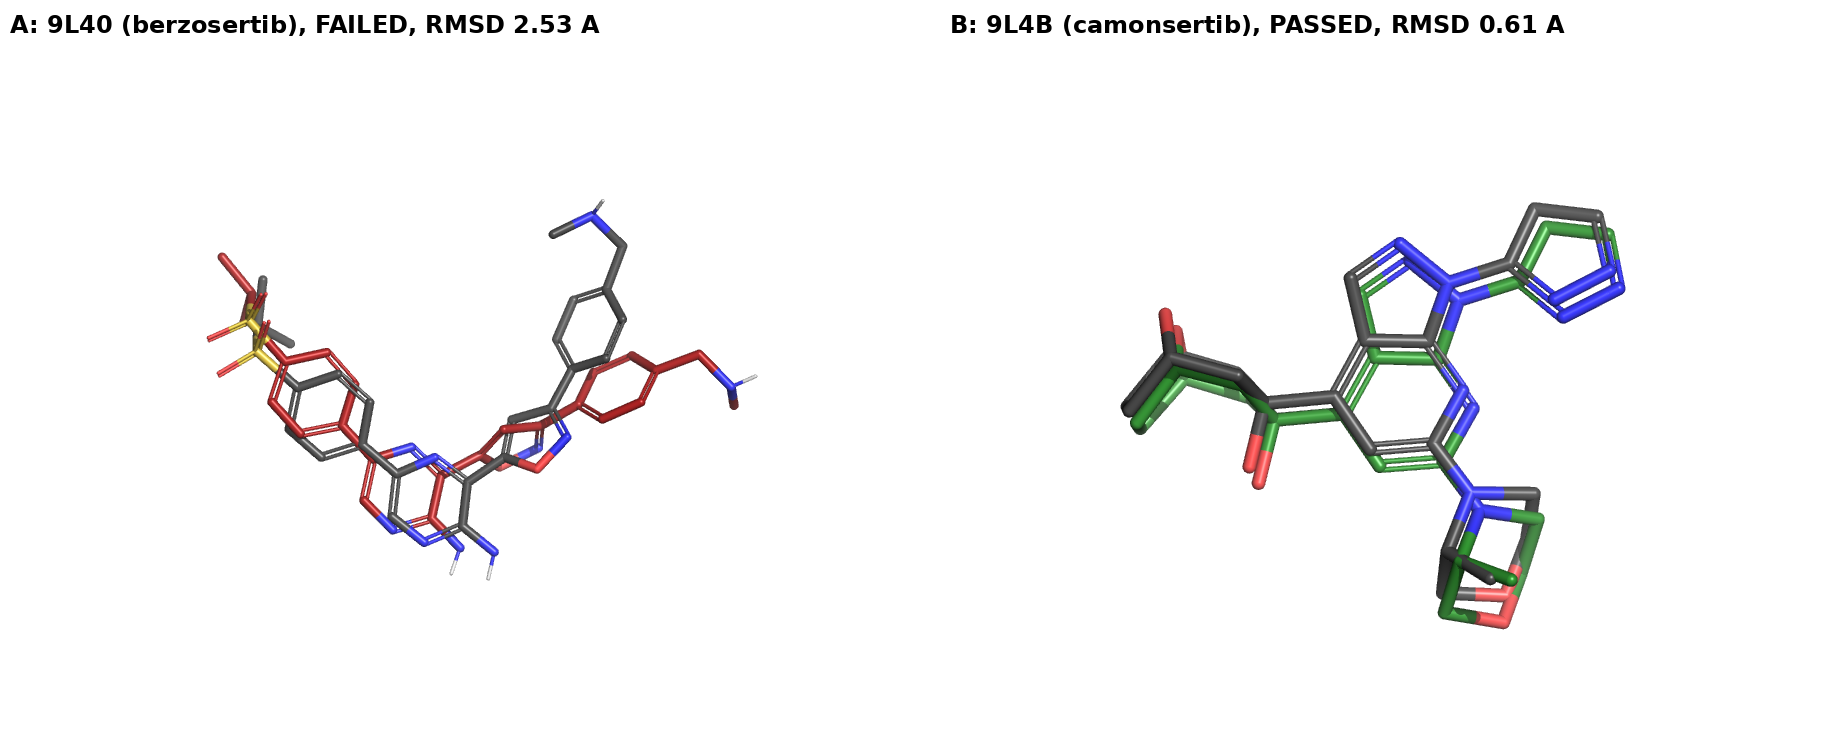
\includegraphics[width=\columnwidth]{figure_redocking_overlay.png}
\caption{Native (grey) vs. redocked (colored) best pose. Left:
9L40/berzosertib (symmetry-corrected RMSD 2.53~\AA{}). Right:
9L4B/camonsertib (0.61~\AA{}).}
\label{fig:overlay}
\end{figure}

\begin{table}[t]
\centering
\caption{Redocking validation (three seeded Vina replicates,
exhaustiveness~32)}
\label{tab:redocking}
\st
\begin{tabular}{lcccl}
\toprule
Structure & Res. (\AA{}) & RMSD (\AA{}) & Pass? & Repro.\ (\AA{})$^a$ \\
\midrule
9L40 (ATR)      & 2.87 & 2.53$\pm$0.01 & \textbf{No} & 0.56 \\
9L4B (ATR)      & 3.20 & 0.61$\pm$0.02 & Yes         & 0.045 \\
2YM8 (CHK1)$^b$ & 2.07 & 0.76$\pm$0.01 & Yes         & 0.078 \\
\bottomrule
\end{tabular}
\vspace{2pt}
{\footnotesize $^a$ Search reproducibility defined as mean pairwise RMSD
between each replicate's best-scoring pose. $^b$ Non-cryo-EM (X-ray
crystallographic) reference structure.}
\end{table}

\begin{table}[t]
\centering
\caption{Minimally processed receptor controls (Open Babel only, no Meeko
deletion)}
\label{tab:receptorcontrols}
\st
\begin{tabular}{lccc}
\toprule
Structure & Open Babel RMSD (\AA{}) & Meeko RMSD (\AA{}) & Pass/fail \\
\midrule
9L40 & 2.59$\pm$0.03 & 2.53$\pm$0.01 & same (fail) \\
9L4B & 0.63$\pm$0.02 & 0.61$\pm$0.02 & same (pass) \\
\bottomrule
\end{tabular}
\end{table}

\subsection{Multi-structure survey}

Table~2 reports results for all 17 structures (full table with residue
inclusion in Supplementary Table~S1). Within this sample, 14 of 17 (82\%)
failed the 2.0~\AA{} threshold; only 9L4B, 2YM8, and one CAK entry (8P75)
passed. No statistically significant monotonic association between reported
resolution and redocking outcome was detected (Spearman $\rho=-0.28$,
$p=0.28$, $n=17$). No statistically significant association between the
evaluated global measure of residue inclusion and redocking outcome was
detected ($r=-0.14$, $p=0.61$, $n=16$). Among the 12 structures with a
reported Q-score, the two passing structures had a lower mean Q-score (0.569)
than the 10 failing structures (0.688); however, with only two passing
Q-scored structures, no statistically interpretable comparison is possible,
and these results should be read as exploratory rather than evidence that
Q-score lacks predictive value. Across the CAK failures, the docked ligand
centroid remained close to its native centroid (1.1--4.1~\AA{}) despite RMSDs
of 5--7~\AA{}, indicating reorientation within the pocket rather than gross
displacement.

The 14 CAK structures derive from a single target system and research group
and therefore represent clustered observations, not 14 independent targets.
Within this single-target series, 13 of 14 structures failed the prespecified
criterion.

\begin{table}[t]
\centering
\caption{Multi-structure survey, sorted by symmetry-corrected RMSD}
\label{tab:survey}
\st
\begin{tabular}{lcccl}
\toprule
Structure & Res. (\AA{}) & RMSD (\AA{}) & Pass? & Q-score \\
\midrule
9L4B (ATR)  & 3.20 & 0.61 & Yes & 0.528 \\
2YM8 (CHK1) & 2.07 & 0.76 & Yes & n/a \\
8P75 (CAK)  & 2.00 & 1.03 & Yes & 0.609 \\
9L40 (ATR)  & 2.87 & 2.53 & No  & 0.553 \\
8P72 (CAK)  & 1.90 & 2.70 & No  & 0.707 \\
8P6Z (CAK)  & 2.10 & 4.84 & No  & 0.705 \\
8P6V (CAK)  & 1.90 & 6.14 & No  & 0.738 \\
8P7L (CAK)  & 2.10 & 6.16 & No  & 0.708 \\
8P74 (CAK)  & 2.20 & 6.67 & No  & 0.628 \\
8P6W (CAK)  & 1.90 & 7.33 & No  & 0.762 \\
\bottomrule
\end{tabular}
\end{table}

\subsection{Exploratory positive control}

The unmodified pipeline passed 8 of 20 (40\%) CASF-2016 subset complexes
selected by prespecified pseudorandom stratified sampling (Table~3). The exact
95\% binomial confidence interval is 19.1--63.9\%. Because failure to reject a
null hypothesis does not establish equivalence, this subset was treated as an
exploratory control rather than evidence that the pipeline is definitively
valid. The 40\% rate was not statistically distinguishable from the literature
Vina value of 58\% on the full 285-complex core set~\cite{zhang2023} (one-sided
binomial $p=0.08$), though this comparison is limited by small sample size and
protocol differences. The 58\% reference value represents Vina performance in a
randomized-ligand redocking experiment and should not be interpreted as a
universal ``Vina success rate,'' as other CASF-2016 evaluations using different
protocols report substantially higher top-pose success rates (Section~S1).

The CAK series (1/14 passed, 7.1\%; exact 95\%~CI 0.2--33.9\%) showed fewer
successful redockings than the exploratory CASF subset (8/20, 40\%). Fisher's
exact test gave $p=0.037$ for the prespecified one-sided comparison (motivated
by the hypothesis that CAK success would be lower than the CASF control) and
$p=0.050$ for the corresponding two-sided comparison. The CASF control did not
reveal an obvious gross failure of the docking implementation, whereas 13 of
14 structures in the sampled CAK series failed the prespecified criterion.

\begin{table}[t]
\centering
\caption{Summary of redocking outcomes}
\label{tab:casf}
\st
\begin{tabular}{lccc}
\toprule
Set & $n$ & Pass (rate) & 95\%~CI \\
\midrule
CASF-2016 subset (exploratory control) & 20 & 8 (40\%)   & 19.1--63.9\% \\
CAK series (single-target)             & 14 & 1 (7.1\%)  & 0.2--33.9\% \\
ATR pair (9L40/9L4B)                   & 2  & 1 (50\%)   & 1.3--98.7\% \\
\bottomrule
\end{tabular}
\end{table}

\subsection{Matched flexible-sidechain analysis}

Five active-site residues within 4.5~\AA{} of native berzosertib (prespecified
from the native complex) were allowed to move with Vina's flexible-sidechain
feature. Box size was held constant at 22~\AA{} for both the flexible run and
its matched rigid control. Allowing the selected active-site side chains to
move partially improved pose reproduction: flexible-sidechain docking reduced
RMSD from a matched rigid control of 4.77$\pm$0.06~\AA{} (22~\AA{} rigid only)
to 3.48$\pm$0.88~\AA{} (22~\AA{} flexible). Sensitivity analyses using 3
residues (3.92$\pm$0.91~\AA{}) and all residues within 5.0~\AA{}
(3.31$\pm$0.94~\AA{}) showed similar partial improvements (Supplementary
Table~S5). These results indicate that local receptor flexibility can
contribute to the observed failure, although the experiment does not partition
receptor conformational effects from other consequences of the flexible-docking
model.

\subsection{Error-propagation comparison}

Docking the 40-compound pilot set against the excluded 9L40 instead of
validated 9L4B produced low rank concordance: Spearman $\rho=0.21$ (bootstrap
95\%~CI $-0.19$ to $0.52$), Kendall~$\tau=0.09$, mean absolute rank
displacement~11.7 positions (max~29), and only 5 of 10 compounds shared
between the two top-10 lists (Table~4). The five shared top-10 compounds were:
camonsertib, ceralasertib, deriv\_002, deriv\_003, and deriv\_019, the same
compounds that occupied the top five ranks in the 9L4B ranking. These results
show that receptor choice can alter compound prioritization within this pilot
set; they do not establish a general loss of screening performance.

\begin{table}[t]
\centering
\caption{Largest rank shifts between 9L40 and 9L4B scoring (matched
three-seed design, $n=40$)}
\label{tab:errorprop}
\st
\begin{tabular}{lccc}
\toprule
Compound & Rank (9L40) & Rank (9L4B) & Shift \\
\midrule
deriv\_017 & 5  & 34 & 29 \\
deriv\_010 & 10 & 39 & 29 \\
deriv\_022 & 32 & 7  & 25 \\
deriv\_033 & 34 & 9  & 25 \\
\bottomrule
\end{tabular}
\end{table}

\subsection{Implications for practice}

Cognate redocking provides a structure-specific quality-control test that can
identify docking failures not apparent from nominal resolution or the evaluated
global map/model metrics. 9L40 and 9L4B were solved in the same study, yet
only the lower-resolution one passed---an inversion that no proxy metric
captured. The observation was reproduced in a separate CAK structure series,
although the CAK structures derive from a single target system and therefore do
not establish target-independent generality. The 13/14 observed failures in the
sampled CAK series should be treated as descriptive evidence within that series
rather than as a kinase-wide failure frequency.

No statistically significant association between the available global
map/model metrics and redocking outcome was detected in this small survey.
Because only two structures with available Q-score measurements passed, the
Q-score analysis in particular was underpowered and should be interpreted as
exploratory. These results support the use of per-structure cognate redocking
as a quality-control step, while systematic multi-target evaluation is required
to determine its general utility.

\subsection{Limitations}

This is a small pilot ($n=17$); the CAK set is a single-target convenience
sample. The global Q-score analysis is underpowered (2 passing structures with
reported Q-scores). Local density-fit metrics were assessed for 9L40/9L4B but
a full per-residue active-site analysis across all 17 structures was not
performed; such an analysis would require uniform local validation-report data
that were not consistently available. No MD, MM-GBSA, or cross-kinase
selectivity was run. Nothing establishes functional modulation---only predicted
binding.

% ======================================================================
\section{Conclusions}

Cognate redocking provides a structure-specific quality-control test that can
identify failures not apparent from nominal resolution or the evaluated global
map/model metrics. Applied to two ATR structures from the same study, the test
passed the lower-resolution one and failed the higher-resolution one, an
inversion that survives box-size sensitivity analysis and is not explained by
allosteric-site proximity. Within a single-target CAK structure series, 13
of 14 entries failed the same criterion. Cognate redocking is a useful
structure-specific QC test that can expose docking failures not obvious from
nominal resolution or the evaluated global map/model metrics, but its
necessity and sufficiency for prospective enrichment require systematic
evaluation. A systematic, multi-target survey is required to establish whether
the proportion of failures observed here is representative of recently
deposited kinase structures generally. All code, data, and structures are
openly available.

% ======================================================================
\section*{Acknowledgements}
[Placeholder]

\section*{Author contributions}
[Placeholder]

\section*{Data availability}
All code, seed and derivative compound tables, redocking validation results, and
pilot docking results are available at
\url{https://github.com/ethanyyy123/research-molecule-editing}. Individual
replicate RMSDs, prepared PDBQT files, and full residue-deletion lists are in
Supplementary Tables S1--S6. Receptor structures are publicly available from
RCSB PDB (9L40, 9L4B, 2YM8) and were retrieved via the AWS Open Data mirror
(\url{s3://pdbsnapshots}).

\section*{Declarations}
\textbf{Conflict of interest:} [Placeholder]

\bibliographystyle{unsrtnat}
\bibliography{refs}

\end{document}